\subsubsection{Производящая функция и полиномы Лежандра}
Полиномы Лежандра применяются при решении задачи Штурма-Лиувилля, тесно связаны с решением уравнения Лапласа $\frac{1}{R}$, R - расстояние точки $M$ от фиксированной $M_0$.\\
\begin{wrapfigure}[8]{l}{0.3\textwidth}
	\centering
	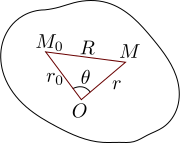
\includegraphics[width=0.3\textwidth]{figLejandr1.pdf}
\end{wrapfigure}
Пусть $r$ и $r_0$ -- радиусы векторы точек $M$ и $M_0$, a $\theta$ - угол между ними. 
Используя теорему косинусов представим $R$ через $r$
\[
    \frac{1}{R} = \frac{1}{\sqrt{r_0^2 + r^2 - 2 r r_0 \cos \theta}}
\]

Рассмотрим два случая
\begin{align*}
    &r > r_0 \quad \frac{r_0}{r} < 1 \quad \frac{r_0}{r} = \rho < 1\\
	&r < r_0 \quad \frac{r_0}{r} < 1 \quad \frac{r}{r_0} = \rho < 1
\end{align*}

\begin{align*}
    &1) \frac{1}{R} = \frac{1}{r \sqrt{1 + \rho^2 - 2 \rho \cos \theta}}\\
	&2) \frac{1}{R } = \frac{1}{r_0 \sqrt{1 + \rho^2 - 2 \rho \cos \theta}}
\end{align*}

\[ 
    \psi (\rho, \theta) = \frac{1}{\sqrt{1 + \rho^2 - 2 \rho \cos \theta}}
\]
Функция
\begin{equation}
    \psi(\rho, z) = \frac{1}{\sqrt{1 + \rho^2 - 2 \rho z}}
    \label{equ:poly}
\end{equation}
называется \textit{производящей функцией} полиномов Лежандра.
\begin{multline}
    \psi (\rho, z) = \left[1 + (\rho^2 - 2 \rho z) \right]^{-\frac{1}{2}} = 1 - \frac{1}{2} (\rho^2 - 2 \rho z) - \frac{1}{2} \left(- \frac{3}{2} \frac{1}{2}\right) (\rho^2 - 2 \rho z)^2 + \ldots = \\= 1 + z \rho + \left( \frac{3}{2}z^2 - \frac{1}{2}\right) + \rho^2 + \ldots
\end{multline}

Получим разложение функции $\psi$ в ряд.
\[
	\psi(\rho, z) = \left[1 + (\rho^2 - 2 \rho z) \right]^{- \frac{1}{2}} = \sum\limits_{n = 0}^{\infty} P_n (z) \rho^n
\]
\begin{equation}
    \psi(\rho, z) = \sum\limits_{n = 0}^{\infty} P_n (z) \rho^n
	\label{equ:polyRow}
\end{equation}
Коэффициенты разложения \eqref{equ:polyRow} при одинаковых степенях $\rho$ образуют \textit{полиномы Лежандра}.

Обратимся к формуле \eqref{equ:poly}
\[z = 1, \quad \psi (\rho, 1 )= (1 + \rho^2 - 2 \rho)^{- \frac{1}{2}} = (1 - \rho)^{-1} = 1 + \rho + \rho^2 + \ldots \Rightarrow P_n(1) = 1\]

В дальнейшем получим рекуррентное соотношение.
\subsubsection{Рекуррентные формулы}
Выведем три рекуррентные формулы.

Продифференциируем $\psi$ по $\rho$
\[
    \derp{\psi}{\rho}{} = \frac{2 \rho - 2 z}{2 (1 + \rho^2 - 2 \rho z)^{\frac{3}{2}}} = \frac{- (\rho - z)}{(1 + \rho^2 - 2 p z)^{\frac{3}{2}}}
\]
\begin{equation}
	(1 + \rho^2 - 2 \rho z) \derp{\psi}{\rho}{} = - (\rho - z) \psi
	\label{equ:poly3}
\end{equation}
Запишем формулу в виде степенного ряда относительно $\rho$, подставив в неё ряд \eqref{equ:polyRow}
\begin{multline*}
    (1 + \rho^2 - 2 \rho z) \left[\ldots + (n - 1) P_{n - 1} \rho^{n - 2} + n P_n \rho^{n - 1} + (n + 1) P_{n + 1} \rho^n + \ldots \right] = \\= - (\rho - z) \left(\ldots + P_{n - 1}\rho^{n - 1} + P_n \rho^n + P_{n + 1} \rho^{n + 1}+ \ldots \right)
\end{multline*}
Приведём подобные 
\[(n + 1) P_{n + 1} + (n - 1) P_{n - 1} - 2 n z P_n = - P_{n - 1} + z P_n\]
\[(n + 1) P_{n + 1} + n P_{n - 1} - (2n + 1) z P_n =0\]
Получим \textbf{первую} рекуррентную формулу
\begin{equation}
    (n + 1) P_{n + 1} - z(2n + 1) P_n + n P_{n - 1} = 0
	\label{equ:poly4}
\end{equation}

Продифференциируем $\psi$ по z.
\[
    \derp{\psi}{z}{} = \frac{\rho \psi}{(1 + \rho^2 - 2 \rho z)}
\]

\begin{equation}
    (1 + \rho^2 - 2 \rho z) \derp{\psi}{z}{} = \rho \psi
\end{equation}

\[
\begin{cases}
   \rho z \psi = z (1 + \rho^2 - 2 \rho z) \derp{\psi}{z}{}\\
   \rho^2 \psi = \rho (1 + \rho^2 - 2 \rho z) \derp{\psi}{z}{}
\end{cases}
\]

\[
    \rho \cancel{(1 + \rho^2 - 2 \rho z)} \derp{\psi}{\rho}{} = (z - \rho) \cancel{(1 + \rho^2 - 2 \rho z)} \derp{\psi}{z}{}
\]

\begin{equation}
    \rho \derp{\psi}{\rho}{} = (z - \rho) \derp{\psi}{z}{}
	\label{equ:poly6}
\end{equation}

В равенство \eqref{equ:poly6} подставляем выражение \eqref{equ:polyRow} 
\begin{multline*}
    \rho \left[\ldots + (n - 1) P_{n - 1} \rho^{n - 2} + n P_n \rho^{n - 1} + (n + 1) P_{n + 1} \rho^n + \ldots \right] =\\ = (z - \rho)\left[\ldots + P_{n - 1}' \rho^{n - 1} + P_n' \rho^n + P_{n +1}' \rho^{n + 1} + \ldots \right]
\end{multline*}
Получили \textbf{вторую} рекурентную формулу
\begin{equation}
    n P_n = zP_n' - P_{n - 1}'
	\label{equ:poly7}
\end{equation}
Имеется
\[
    \rho \derp{}{\rho}{} (\rho \psi) = \rho^2 \derp{\psi}{\rho}{} + \rho \psi
\]
\[
    \rho (\rho \psi) = \rho (z - \rho) \derp{\psi}{z}{} + (1 + \rho^2 - 2 \rho z) \derp{\psi}{z}{}
\]

Снова используем \eqref{equ:polyRow}.
\[
    \rho \psi = \rho (\ldots + P_{n - 1} \rho^{n - 1} + P_n \rho^n + P_n + \rho^{n + 1}) = \ldots + P_{n - 1} \rho^{n } P_n \rho^{n + 1} P_{n + 1}\rho^{n + 1}
\]
\[ 
    \derp{(\rho \psi)}{}{} = (\ldots + )
\]
\[
    \derp{\psi}{z}{} (\rho z - \rho^2+ 1 \rho^2 - 2 \rho z) = (1 \rho z) \derp{\psi}{z}{} = (1 - \rho z) (P_{n - 1}' \rho^{n - 1} + P_n' \rho^n + P_{n + 1}' \rho^{n+1} + \ldots)
\]
\[
    n P_{n - 1}\rho^n + (n + 1) P_n \rho^{n + 1} + (n + 2) P_{n + 1} \rho^{n + 2} = P_n' \rho^n - z P_{n - 1}' \rho^n + \ldots
\]
Получаем \textbf{третью} рекуррентную формулу
\begin{equation}
    n P_{n - 1} = P_n' - z P_{n - 1}'
	\label{equ:poly8}
\end{equation}
\subsubsection{Уравнение Лежандра}


%Для этого исключим из систем  \eqref{equ:poly7} и \eqref{equ:poly8} $P_{n - 1}$ и $P_{n - 1}'$. \\

%Сначала подставим $P_{n - 1}'$ из \eqref{equ:poly7} в \eqref{equ:poly8}
%\[
%   P_{n - 1}' = z P_n ' - n P_n
%\]
%\[
%    n P_{n -1 } = P_n ' - z \left[ z P_n ' - n P_n \right]
%\]
%\[
 %   n P_{n - 1} = (1 - z^2) P_n ' + n z P_n
%\]
%Затем продифференциируем последнее равенство по $z$ и ещё раз применим \eqref{equ:poly7} для $P_{n -1 }$
%\[
%    n P_{n - 1}' = - 2 z P_n' + (1 - z^2) P_n'' + n P_n + n z P_n '    
%\]
%\[
%    n (z P_n' - n P_n) = (n - 2) z P_n ' + (1 - z^2) P_n '' + n P_n
%\]
%\[
 %   (1 - z^2) P_{n}'' - 2 z P_n' + n(n + 1)P_n = 0
%\]
%Переобозначим
%\begin{equation}
 %   (1 - z^2) y'' - 2 z y' + n (n + 1)y =0
%	\label{equ:polyLejandr}
%\end{equation}
%Уравнение \eqref{equ:polyLejandr} называется полиномом Лежандра.\\
%Эквивалентная запись 
%\[
%    \der{}{z}{}\left[ (1 - z^2) \der{y}{z}{}\right] + n (n + 1) y = 0
%\]
\setcounter{equation}{0}
Найдём дифференциальное уравнение, решением которого явялется $P_n(z).$
%\begin{equation}
%	\der{}{z}{} \left[(1 - z^2) \der{y}{z}{} \right] + n(n + 1)y = 0
%	\label{equ:AttachedLajandr1}
%\end{equation}
%\[
%	y = P_n(z)
%\]
Реккурентные соотношения для полиномов Лежандра:
\begin{equation}
	(n + 1) P_{n + 1} (z) - z (2n + 1) P_n(z) + n P_{n - 1} (z) = 0
	\label{equ:AttachedLajandr2}
\end{equation}
\begin{equation}
	n P_n (z) - z P_n'(z) + P_{n - 1}(z) = 0
	\label{equ:AttachedLajandr3}
\end{equation}
\begin{equation}
	n P_{n - 1}(z) - P_n'(z) + z P_{n - 1}' (z) = 0
	\label{equ:AttachedLajandr4}
\end{equation}

\[
    \int\limits_{-1}^1 P_n(z) P_m (z) \, dz = 
	\begin{cases} 
		0 & n \neq m \\ 
		\frac{2}{2n + 1} & n = m 
	\end{cases}
\]
%\textit{при условии ограниченности}
%\begin{equation}
%	\abs{y (\pm 1)} < \infty.
%	\label{equ:AttachedLajandr2}
%\end{equation}

%\[
%    P_n(z) = \derp{y}{z}{n} = C \cdot \der{}{z}{n} [(z^2 - 1)^n]
%\]

Рассмотрим дифференциальную форму полиномов Лежандра:
\[
    y = (z^2 - 1)^n; \qquad \der{y}{z}{} = 2 n z (z^2 - 1)^n
\]

\[
    \der{y}{z}{}(z^2 - 1) - 2 n z y = 0
\]
Продифференциируем полученное уравнение $(n + 1)$ раз:
\[
    \der{}{z}{n + 1} \left[(z^2 - 1) \der{y}{z}{} - 2 n \der{}{z}{n + 1} (z y(z))\right] = 0
\]
\begin{align*}
	(u \cdot v)' &= u' v + u v'\\
	(u \cdot v)'' &= u'' c + 2 u' v' + v''\\
	(u \cdot v)''' &= u''' v + 3 u'' v' + 3 u' v '' + v'''
\end{align*}
Тогда 
\begin{equation}
	(u \cdot v)^n = u^{(n)} v + n u^{(n - 1)} v' + \frac{n(n - 1)}{2} u^{(n - 2)} + \ldots + u v^{(n)}
	\label{equ:AttachedLajandr5}
\end{equation}
\[
    \left[\der{}{z}{n + 2} (z^2 - 1) + (n + 1) \der{y}{z}{n+1} 2 z +n(n + 1) \der{y}{z}{n} \right] - 2 n \left[\der{y}{z}{n + 1} z + (n + 1) \der{y}{z}{n}  \right] = 0
\]

\[
    (z^2 - 1) \der{y}{z}{n + 2} + \der{y}{z}{n + 1} [\cancel{2 nz} + 2z - \cancel{2 nz}] + \der{y}{z}{n}[n^2 + n - 2n^2 - 2n] = 0
\]
\begin{equation}
	(1 - z^2) \der{y}{z}{n + 2} - 2 z \der{y}{z}{n + 1} + n(n + 1) \der{y}{z}{n} = 0
	\label{equ:AttachedLajandr6}
\end{equation}
Пусть $\der{y}{z}{n} = P_n$, тогда
\[
    (1 - z^2) \der{P_n}{z}{2} - 2 z \der{P_n}{z}{} + n(n + 1)P_n = 0
\]
Получили \textit{дифференциальное уравнение Лежандра}, которому удовлетворяет $P_n$:
\begin{equation}
    \der{}{z}{} \left[(1 -z^2) \der{P_n}{z}{} \right] + n (n + 1) P_n = 0
	\label{equ:equLejandr}
\end{equation}
где $P_n$ --- полиномы Лежандра:
\[
    P_n(z) = \der{y}{z}{n} = C \der{}{z}{n} \left[(z^2 - 1)^n \right]
\]
так как $y = (z^2 - 1)^n$, а по свойствам полиномов Лежандра $P_n(1) = 1$

\begin{align*}
    \der{}{z}{}\left[(z^2 - 1)^n \right] &= 2 z (z^2 - 1)^{n - 1} n\\
    \der{}{z}{2} \left[(z^2 - 1)^n \right] &= 2 n(z^2 - 1)^{n - 1} + 2 n (n - 1)z^2 (z^2 - 1)^{n - 2}\\
    \der{}{z}{n} \left[(z^2 - 1)^n \right] &= 2^n z^n n (n - 1)(n - 2) \ldots (z^2 - 1) + a(z^2 - 1) z^{n - 1} +b(z^2 - 1)^2 z^{n - 2}
\end{align*}
Тогда при $z = 1$
\[
    P_n(1) = C \der{}{z}{n} \left[ (z^2 - 1)^n \right] \bigl|_{z = 1} = C 2^n n! = 1
\]
и следовательно
\[
    C = \frac{1}{2^n n!}.
\]
Полиномы Лежандра можно представить в дифференциальной форме
\begin{equation}
    P_n(z) = \frac{1}{2^n n!} \der{}{z}{n} \left[(z^2 - 1)^n \right]
    \label{equ:Rodriger}
\end{equation}
Формула \eqref{equ:Rodriger} называется \textit{формулой Родригера.}\\
\subsubsection{Ортогональность полиномов Лежандра}\label{que:28}
Докажем ортогональность полиномов Лежандра на отрезке $[-1, 1]$

\begin{align*}
    &(1 - z^2) P_n'' - 2 z P_n + n (n + 1) P_n = 0 | P_m(z) dz\\
	&(1 - z^2) P_m'' - 2 z P_m + n (m + 1) P_m = 0 | P_n(z) dz
\end{align*}

\[
    \int\limits_{-1}^1 \left\{ P_m \der{}{z}{} \left((1 - z^2) \der{P_n}{z}{}\right) + n (n + 1) P_n P_m - P_n \der{}{z}{} \left((1 - z^2) \der{P_n}{z}{}\right) - m (m + 1) P_n P_m\right\} \, dz
\]
От первого и третьего слагаемого возьмём интеграл по частям

Если $n \neq m$ интеграл $= 0$
\[
    \int\limits_{-1}^1 P_n P_m \,dz = \begin{cases} 0 & n \neq m \\ \neq 0 & n = m \end{cases}
\]

\[
    P_n(z) = a_{nn} z^n + a_{n n - 1} z^{n - 2} + \ldots
\]
Полиномы Лежандра содержат только чётные, либо только нечётные коэффициенты степени $z$
\[
    P_{n-1}(z) = a_{n-1n-1} z^{n-1} + a_{n-1 n - 2} z^{n - 3} + \ldots
\]
Из равенства \eqref{equ:poly4} 
\[
    (n + 1) a_{n+1 n + 1} - (2 n + 1) a_{nn} = 0
\]

Теперь построим такую функцию
\[
    Q(z) = P_n(z) - \frac{a_{nn}}{a_{n - 1 n + 1}z P_{n - 1} (z)} = b_1 z^{n -2} + b_2 z^{n - 4} = \sum\limits_{n = 0}^{n - 2} b_n P_k(z)
\]

\begin{multline}
    N_n = \int\limits_{-1}^{1} P_n(z) P_n(z) \, dz = \int\limits_{-1}^1 P_n(z) \left(Q(z) + \frac{a_nn}{a_{n - 1}} z P_{n - 1}\right) \, dz = \\
	= \int\limits_{-1}^1 P_n Q (z) \, dz + \frac{a_nn}{a_{n - 1 n - 1}} \int\limits_{-1}^1 P_n z P_{n - 1} \, dz
\end{multline}

Воспользуемся равенством \eqref{equ:poly4}
\[
   z P_n = \frac{n P_{n - 1} + (n + 1) P_{n + 1}}{2n + 1}
\]
Получаем
\[
    N_n \int\limits_{-1}^1 P_n(z) P_n (z) \, dz = \frac{a_{nn}}{a_{n -1 n - 1}} \int\limits_{-1}^1 P_{n - 1} \left( \frac{n P_{n - 1} + (n + 1) P_{n + 1}}{2n + 1} \right)\, dz = \frac{a_{nn}}{ a_{n - 1 n - 1} \frac{n}{2 n + 1}} \int\limits_{-1}^1 P_{n - 1}^2 \, dz
\]

\[
    N_n = \frac{2 n - 1}{2 n + 1} N_{n - 1}
\]

\begin{align*}
    &N_0 = \int\limits_{-1}^1  dz = 2\\
    &N_1 = \int\limits_{-1}^1 z^2 dz = \frac{2}{3}\\
    &N_2 =  \frac{2}{5}\\
    &N_3 =  \frac{3}{7}
\end{align*}

По аналогии
\[
    N_n = \frac{2}{2 n + 1}
\]





